\documentclass[11pt]{article}
\usepackage[margin=1in]{geometry}
\usepackage{amsmath, amssymb, amsthm}
\usepackage{physics}
\usepackage{bm}
\usepackage{hyperref}
\usepackage{graphicx}
\usepackage{enumitem}
\usepackage{siunitx}
\usepackage{mathtools}
\usepackage{braket}
\usepackage{quantikz}
\usepackage{tikz}
\usetikzlibrary{arrows.meta,calc}
\usepackage{MnSymbol,wasysym}
\newenvironment{summary}{\par\noindent\textbf{Summary.} }{\par}

\title{CSCI-739 Quantum Machine Learning \\[4pt] \large Homework 4}
\date{}

\begin{document}
\maketitle

\begin{center}
\textit{You made it, team. This homework continues our exploration from expressivity to practicality: from the theoretical foundation of quantum neural networks to their real implementation limits. You’ll confront how quantum encodings shape function classes (P1), how depth affects performance in both classical and quantum learning (P2), and—through the bonuses—how hardware, state complexity, and simulation feasibility bound what’s possible on current machines. Each problem is a lens on scalability, trainability, and the physics of information. You got this. \smiley{}}
\end{center}

\vspace{1em}
\noindent
\textbf{Structure overview:}
\begin{itemize}
  \item \emph{P1:} Theoretical expressivity and the universal approximation property of QNNs.
  \item \emph{P2:} Empirical study of depth and performance in classical vs. quantum neural networks.
  \item \emph{Bonus A:} The “spooky” diagonal Hamiltonian—analytical vs.\ VQE ground state scaling.
  \item \emph{Bonus B:} The complexity hierarchy of quantum state preparation.
  \item \emph{Bonus C:} Multivariate sine regression under increasing input dimension and depth.
\end{itemize}
Use lectures, notes, the internet and each other to research more on the problems and  conquer this homework, team! Have fun \smiley{}! Also:
% ============================================
\newpage


\begin{figure}[h!]
\centering
\vspace{1em}
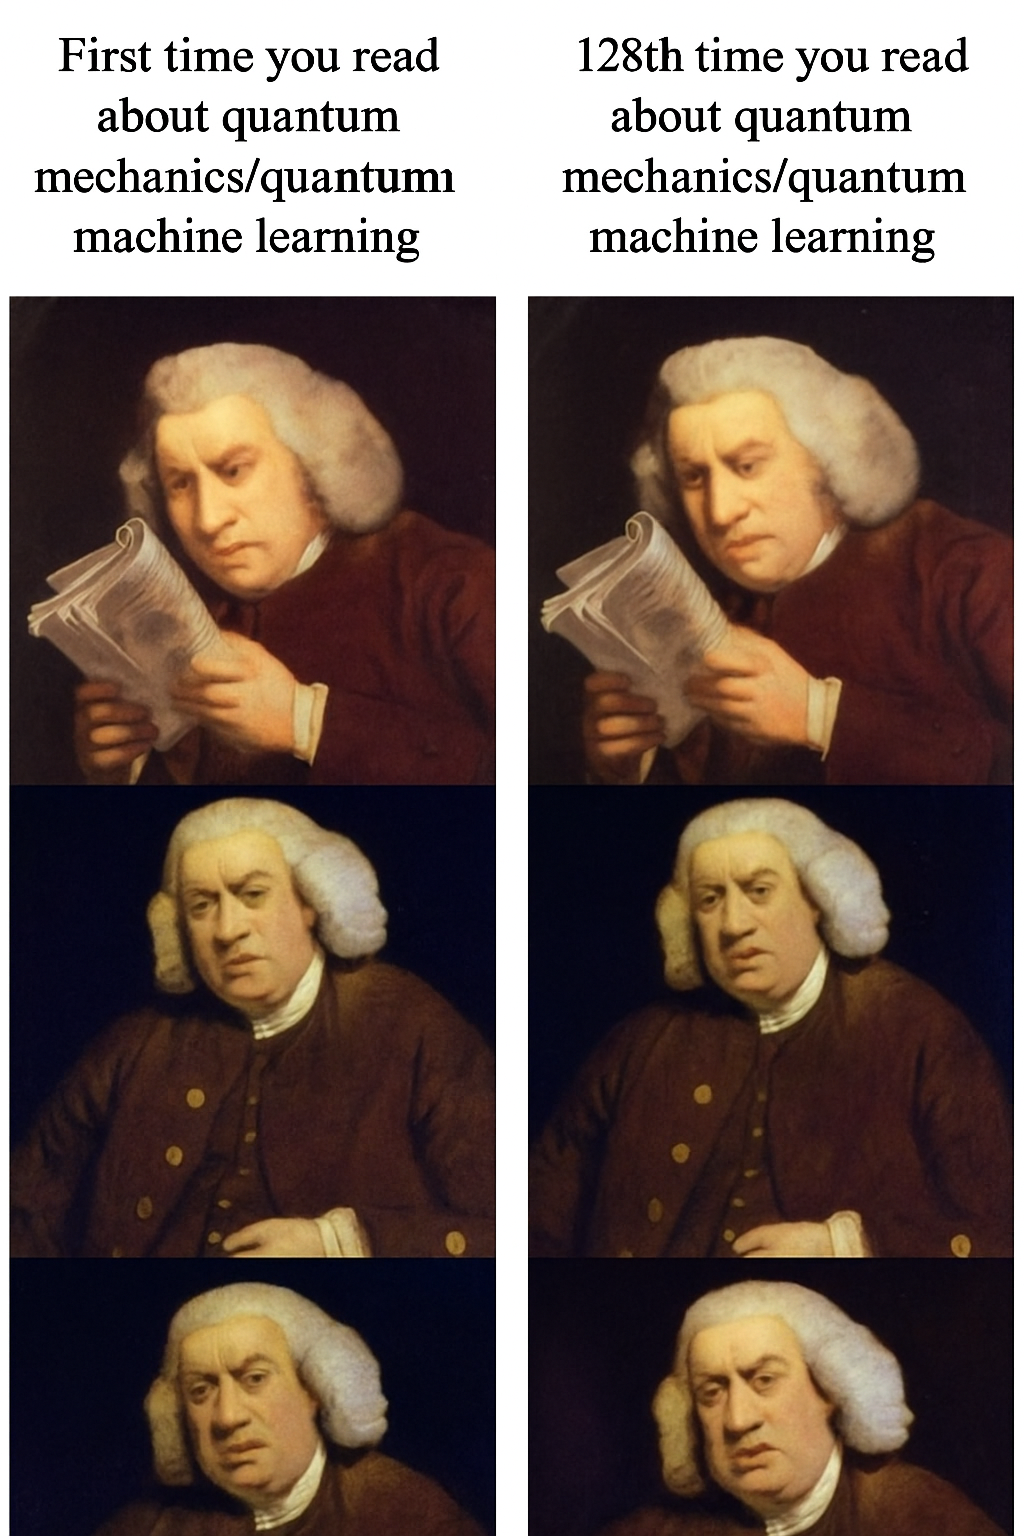
\includegraphics[width=0.75\textwidth]{quantumvogt2.png}
\vspace{0.5em}
\end{figure}

\section*{Problem 1 — Expressivity and Universal Approximation in Quantum Neural Networks (50 pts)}

\begin{summary}
We study how data encodings and parameterized unitaries determine the expressivity of quantum neural networks (QNNs). You will derive conditions under which a QNN can approximate nonlinear functions over classical inputs, compare encoding choices, and connect these results to the universal approximation theorem for classical neural networks.
\end{summary}

A general QNN defines the function
\[
f_{\mathrm{QNN}}(x;\boldsymbol{\theta})
\;=\;
\bra{0}^{\otimes n}\,
U_\phi(x)^\dagger
\,U(\boldsymbol{\theta})^\dagger\,
M\,
U(\boldsymbol{\theta})\,
U_\phi(x)
\,\ket{0}^{\otimes n},
\]
where
\begin{itemize}
\item $x\in\mathbb{R}^d$ is the classical input vector,
\item $U_\phi(x)$ is the \textbf{encoding unitary} (basis, angle, or amplitude encoding),
\item $U(\boldsymbol{\theta})$ is the \textbf{trainable ansatz} of parameterized gates,
\item $M$ is the measurement observable (often $Z$ or $Z_i$),
\item and $f_{\mathrm{QNN}}(x;\boldsymbol{\theta})\in[-1,1]$ is the predicted value.
\end{itemize}

\begin{enumerate}[label=(\alph*)]
\item \textbf{Encoding and expressivity.}  
Compare basis encoding $\ket{x}\mapsto\ket{x}$ and angle encoding $\ket{0}\mapsto R_y(\pi x)\ket{0}$.  
Show that for angle encoding, $f_{\mathrm{QNN}}(x;\theta)$ becomes a trigonometric polynomial in $x$. Discuss why this nonlinearity increases representational capacity relative to basis encoding.

\item \textbf{Simple one-qubit example.}  
Let $U_\phi(x)=R_y(\pi x)$, $U(\theta)=R_y(\theta)$, and $M=Z$.  
Compute
\[
f_{\mathrm{QNN}}(x;\theta)
=\bra{0}R_y(-\pi x)R_y(-\theta)Z R_y(\theta)R_y(\pi x)\ket{0}.
\]
Simplify analytically and describe the functional form of $f_{\mathrm{QNN}}(x;\theta)$.

\item \textbf{Universal approximation.}  
Discuss qualitatively how multi-qubit, layered QNNs can approximate arbitrary continuous functions $f:\mathbb{R}^d\to[-1,1]$, analogous to classical feedforward networks.  
Relate this to the idea that as circuit depth grows, the space of realizable trigonometric combinations becomes dense in $C([0,1]^d)$.

\item \textbf{Relationship between classical and quantum NN.}   
Why would a QNN restricted to linear encodings and shallow layers collapse to a classical linear model?
\end{enumerate}

% ============================================
\newpage
\section*{Problem 2 — Classical vs.\ Quantum Neural Networks on a Sine Function (50 pts)}

\begin{summary}
You will implement both a classical and quantum neural network to learn a one-dimensional sine function.  
By varying the number of layers, you will observe when additional depth helps and when it hurts, illustrating the interplay between expressivity and trainability.
\end{summary}

\paragraph{Target function.}
\[
y(x) = \sin(2\pi x), \qquad x\in[0,1].
\]

\paragraph{Dataset.}
Sample $N_{\text{train}}=64$ uniformly spaced training points and $N_{\text{test}}=256$ test points.

\paragraph{Objective (common for both models).}
\[
\mathcal{L} = \frac{1}{N}\sum_{i=1}^N \big(\hat{y}(x_i;\boldsymbol{\theta}) - y(x_i)\big)^2,
\]
where $\hat{y}$ is the output of the model (let it be classical or quantum).
\subsection*{Classical model (MLP baseline)}
Use a multilayer perceptron with 1 input, 1 output, and hidden layers of width $\ge 16$ with $\tanh$ activation.  
Train for $L\in\{1,2,4,8\}$ hidden layers using Adam or another optimizer.  
Plot train/test MSE vs.\ epochs and compare performance across $L$.

\subsection*{Quantum model (QNN)}

\paragraph{Encoding.}
Angle encoding identical in structure to Problem 1:
\[
U_\phi(x) = R_y(\pi x).
\]

\paragraph{Ansatz structure (one-qubit case).}
Each layer applies a rotation followed by an optional entangler (identity here):
\[
U(\theta_1,\ldots,\theta_L) = R_y(\theta_L)\cdots R_y(\theta_1).
\]

\paragraph{Model output.}
\[
f_{\mathrm{QNN}}(x;\boldsymbol{\theta})
=
\bra{0}U_\phi(x)^\dagger U(\boldsymbol{\theta})^\dagger Z U(\boldsymbol{\theta})U_\phi(x)\ket{0}.
\]
Estimate $\langle Z\rangle$ by shot-based sampling ($S$ shots).  
Convert to probability $p=(1-\langle Z\rangle)/2$ if needed.

\paragraph{Optimization.}
Minimize $\mathcal{L}_{\text{QNN}}$ via parameter-shift gradient:
\[
\frac{\partial \mathcal{L}}{\partial \theta}
=\frac{1}{2}\big[\mathcal{L}(\theta+\tfrac{\pi}{2})-\mathcal{L}(\theta-\tfrac{\pi}{2})\big].
\]

\paragraph{Experiments.}
For $L\in\{1,2,4,8\}$:
\begin{itemize}
\item Train both the MLP and QNN on the same data.
\item Compare MSE and convergence behavior.
\item Discuss why depth helps initially but may cause vanishing gradients in QNNs.
\end{itemize}

\paragraph{Deliverables.}
For both the classical and quantum simulations plots of predicted vs.\ true $\sin(2\pi x)$, loss vs.\ epochs, and gradient norms vs. \ epochs. Notice anything interesting? \smiley{}

% ============================================
\newpage
\section*{Bonus A (the spooky question that disappeared from HW3 and returned to HW4) — Ground States for a Purely Diagonal $n$-Qubit Hamiltonian with Indexed Spectrum (25 pts)}

\begin{summary}
We study an $n$-qubit Hamiltonian that is strictly diagonal in the computational basis and whose diagonal entries increase with the integer index of the basis state. You will (i) derive the spectrum and ground state analytically, (ii) compare classical storage scaling $2^n$ vs.\ quantum $n$, and (iii) implement a minimal VQE that estimates the ground energy by sampling $Z$-basis measurements. This problem highlights how even simple diagonal Hamiltonians illustrate exponential classical–quantum representational gaps.
\end{summary}

\textbf{Definition (diagonal by basis index).}  
Label computational-basis states $\ket{j}$ by $j\in\{0,1,\dots,2^n-1\}$ with binary expansion. Define
\[
H_n=\mathrm{diag}(E_j)_{j=0}^{2^n-1},\qquad E_j=j+1.
\]
All off-diagonal elements are zero.

\begin{itemize}
  \item A $Z$-basis measurement returns a bitstring
  \[
  \mathbf{b}=(b_{n-1}\dots b_1b_0)\in\{0,1\}^n,
  \]
  corresponding to integer $j=\sum_{i=0}^{n-1}2^{\,i}b_i$.
  \item The random variable \(J\) (“measurement outcome as integer”) has
  \[
  p_j=\Pr(J=j)=|\braket{j}{\psi}|^2.
  \]
\end{itemize}

\[
\langle J\rangle=\sum_{j=0}^{2^n-1}j\,p_j,
\quad
E_n(\boldsymbol{\theta})=\sum_j(j+1)p_j=\langle J\rangle+1.
\]
For $S$ shots:
\[
\widehat{\langle J\rangle}=\frac{1}{S}\sum_{t=1}^{S}j^{(t)},
\qquad
\widehat{E}_n=\widehat{\langle J\rangle}+1,
\quad
\mathrm{Var}[\widehat{\langle J\rangle}]=\frac{\mathrm{Var}(J)}{S}.
\]

\begin{enumerate}[label=(\alph*)]
\item \textbf{Eigenvalues and eigenstates.}  
Show that $\ket{j}=e_{j+1}$ (standard basis) is an eigenvector with eigenvalue $E_j=j+1$.

\item \textbf{Ground state and energy, and classical computational cost.}  
Show $E_0^{(\mathrm{an})}(n)=1$ with ground state $\ket{0\cdots0}=e_1$.  

Now reason about classical feasibility:  
the Hamiltonian is $2^n\times2^n$ ($4^n$ real entries).  
For $n=10$, this is $\sim10^6$ entries; for $n=40$, $\sim10^{24}$—impossible even on supercomputers.  
A molecule such as $\mathrm{Fe}_2\mathrm{S}_2$ or a protein fragment mapped to $n\!\sim\!40$ logical qubits has a $2^{40}\!\times\!2^{40}$ Hamiltonian—far beyond HPC capacity.  
Explain why an $n$-qubit quantum device represents these amplitudes implicitly, motivating VQE.

\item \textbf{Classical vs.\ quantum scaling.}  
Plot $2^n$ vs.\ $n$ for $n=1,\dots,n_{\max}$ in the case of for $n=1,...,40$. in a log scale. Comment on the amount of classical versus quantum resources one needs to represent the $n$ two-level qubit system. Also, comment on the feasibility of finding the lowest energy and corresponding ground state in the case of $n=40$, leveraging state-of-the-art numerical eigenvector/eigenvalue solvers. Do we have a problem \smiley{}? How many qubits would you need to try to approximate the lowest energy state and the corresponding ground state?  

% \item \textbf{VQE formulation.}  
% \[
% E_n(\boldsymbol{\theta})=\sum_{j}(j+1)|\braket{j}{\psi}|^2
% =\langle j\rangle_{\boldsymbol{\theta}}+1.
% \] \paragraph{Defining $\langle j \rangle$ and $\widehat{\langle j \rangle}$.}

% Let the post-ansatz quantum state be
% \[
% \ket{\psi(\boldsymbol{\theta})} = U(\boldsymbol{\theta})\ket{0}^{\otimes n}.
% \]
% When measured in the computational ($Z$) basis, the outcome is a bitstring
% \[
% \mathbf{b} = (b_{n-1}\dots b_1b_0)\in\{0,1\}^n,
% \]
% which corresponds to an integer
% \[
% j = \sum_{i=0}^{n-1} 2^i\, b_i.
% \]
% We denote this random variable by $J$.

% The \textbf{true expectation value} of this index under the state $\ket{\psi(\boldsymbol{\theta})}$ is
% \[
% \boxed{
% \langle j \rangle_{\boldsymbol{\theta}}
% =
% \lim_{S \to \infty}
% \frac{1}{S}\sum_{t=1}^{S} j^{(t)}
% =
% \sum_{j=0}^{2^n - 1} j \, |\braket{j}{\psi(\boldsymbol{\theta})}|^2,
% }
% \],
% where
% \[
% \boxed{
% \langle j \rangle
% = 
% \lim_{S \to \infty}
% \frac{1}{S}\sum_{t=1}^{S} j^{(t)}.
% }
% \]
% This represents the mean integer outcome that would be observed over infinitely many $Z$-basis measurements.

% \vspace{0.5em}
% In a real (or simulated) experiment with $S$ measurement shots, we form the \textbf{empirical estimator}
% \[
% \boxed{
% \widehat{\langle j \rangle}_{\boldsymbol{\theta}}
% =
% \frac{1}{S}\sum_{t=1}^{S} j^{(t)},
% }
% \]
% where each $j^{(t)}$ is the integer label of the $t$-th observed computational-basis outcome.

% \vspace{0.5em}
% The statistical uncertainty of this finite-shot estimator obeys
% \[
% \mathrm{Var}\big[\widehat{\langle j \rangle}\big]
% =
% \frac{\mathrm{Var}(J)}{S},
% \qquad
% \text{where}\quad
% \mathrm{Var}(J)
% =
% \langle j^2 \rangle - \langle j \rangle^2.
% \]
% to estimate them: 
% \noindent
% In practice, given $S$ measurement outcomes $j^{(1)},\dots,j^{(S)}$:
% \[
% \widehat{\langle j \rangle} = \frac{1}{S}\sum_{t=1}^{S} j^{(t)}, 
% \quad
% \widehat{\langle j^2 \rangle} = \frac{1}{S}\sum_{t=1}^{S} \big(j^{(t)}\big)^2,
% \]
% \[
% \widehat{\mathrm{Var}}(J)
% =
% \widehat{\langle j^2 \rangle} - \big(\widehat{\langle j \rangle}\big)^2,
% \qquad
% \widehat{\mathrm{Var}}\!\big[\widehat{\langle j \rangle}\big]
% =
% \frac{\widehat{\mathrm{Var}}(J)}{S}.
% \]

% \vspace{0.5em}
% Finally, the \textbf{estimated energy} for the variational quantum eigensolver (VQE) is
% \[
% \widehat{E}_n(\boldsymbol{\theta})
% =
% \widehat{\langle j \rangle}_{\boldsymbol{\theta}} + 1,
% \]
% which serves as the cost function to be minimized during optimization.

% Estimate $\widehat{\langle j\rangle}$ from $Z$-basis shots.

\item \textbf{Ansatz (no entanglers).}  
\[
\ket{\psi(\boldsymbol{\theta})}=\bigotimes_{i=1}^n R_y(\theta_i)\ket{0}.
\]
Minimize $\widehat{E}_n=\widehat{\langle j\rangle}+1$ in two cases. First, analytically find the $\theta^*$ which minimizes the functional; and in the second case and also find minimize the functional using some  numerical optimization approach. Do you get the same answer between the two? Is the answer you found what you expect?

For context: Let $b_i^{(t)} \in \{0,1\}$ denote the measurement outcome of the $i$-th qubit on the $t$-th shot, 
where $i=0$ corresponds to the \textbf{least significant bit (LSB)} of the binary representation of the measured integer $j^{(t)}$. 
Formally, each $n$-qubit computational-basis outcome $\mathbf{b}=(b_{n-1}\dots b_1 b_0)$ corresponds to the integer
\[
j^{(t)} = \sum_{i=0}^{n-1} 2^{\,i}\, b_i^{(t)},
\]
where $b_0$ is the LSB (the rightmost bit) and $b_{n-1}$ is the most significant bit (MSB).

Define $n^{(i)}_1 = \sum_{t=1}^S b_i^{(t)}$ as the number of shots in which qubit $i$ is measured in the $\ket{1}$ state, 
and $\hat{p}_i = n^{(i)}_1 / S$ as the corresponding empirical probability. Then, because expectation values are linear,
\[
\boxed{
\widehat{\langle j \rangle}
= \sum_{i=0}^{n-1} 2^{\,i}\,\hat{p}_i
= \sum_{i=0}^{n-1} 2^{\,i}\,\frac{n^{(i)}_1}{S}.
}
\]
This bitwise expression is equivalent to computing
\[
\widehat{\langle j\rangle}
=\frac{1}{S}\sum_{t=1}^{S} j^{(t)}
=\sum_{j=0}^{2^n-1} j\,\frac{c_j}{S},
\]
where $c_j$ is the total number of times the outcome $j$ is observed among the $S$ shots.

\item \textbf{Comparison across sizes.}  
Plot $\widehat{E}_n^{(\mathrm{vqe})}$ vs.\ $E_0^{(\mathrm{an})}(n)=1$ and discuss variance growth with $n$.

\item \textbf{Resource limits.}  
Track time/memory vs.\ $n$ and identify when simulation bottlenecks appear. What $n$ value does QISKIT complain on? Did you get to $40$ \smiley{} for this extremely simple version of a ground state problem where we know what the answer is? Comment on the difficulty of a classical computer to simulate the quantum system in general, and how this motivates the interest in VQC for determining the lowest energy and corresponding ground state of a Hamiltonian $H$.

\item \textbf{(Optional) Real hardware shot sweep.}  
Run for $S\in\{1,10,100\}$ and confirm $\mathrm{Var}[\widehat{\langle j\rangle}]=\mathrm{Var}(J)/S$.
\end{enumerate}

% ============================================
\newpage
\section*{Bonus B — The Complexity of Quantum State Preparation (25 pts)}

\begin{summary}
We examine the difficulty of preparing quantum states. Although any normalized vector exists mathematically, preparing it physically by a finite circuit can range from trivial to impossible. You will reason through three regimes: (i) easily preparable states, (ii) exponentially hard states, and (iii) physically impossible states. This reveals how state-preparation complexity limits QNN and VQE ansätze. For each example  make the circuit and in terms of the parameter $n$ in big $\mathcal{O}$ notation give the depth of the the gate circuit depth required to prepare the state e.g. polynomial, exponential, or impossible. In the case of impossible, explain what physical law, rule, or concept makes the state not constructable \smiley{}.
\end{summary}

\begin{enumerate}[label=(\alph*)]
\item \textbf{Easily preparable states.}
\begin{itemize}
  \item \textbf{Uniform superposition:}
  \[
  \ket{\psi_{\mathrm{unif}}}=\frac{1}{\sqrt{2^n}}\sum_{j=0}^{2^n-1}\ket{j}.
  \]
  
  \item \textbf{GHZ state:}
  \[
  \ket{\mathrm{GHZ}_n}=\frac{1}{\sqrt{2}}\big(\ket{0}^{\otimes n}+\ket{1}^{\otimes n}\big).
  \]
  
\end{itemize}

\item \textbf{Computationally hard states.}
\begin{itemize}
  \item \textbf{Haar random:}
  \[
  \ket{\psi_{\mathrm{Haar}}}=\sum_{j=0}^{2^n-1}c_j\ket{j}, \quad c_j\sim\mathcal{N}_{\mathbb{C}}(0,1), \ \sum_j|c_j|^2=1.
  \]

  \item \textbf{Frustrated spin-glass ground state:}
  \[
  H=\sum_{\langle i,j\rangle}J_{ij}Z_iZ_j+\sum_i h_iZ_i,
  \]
Where $Z_i = I \otimes I \otimes .... Z ...I \otimes I  $  e.g. a Z gate on the $i$-th qubit.

 
\end{itemize}

\item \textbf{Impossible states.}
\begin{itemize}
  \item Non-normalizable: e.g.\ position eigenstate $\ket{x}$.
  \item No-cloning: cannot prepare $\ket{\psi}\otimes\ket{\psi}$ from unknown, general psi, $\ket{\psi}$.
  \item Non-Hermitian eigenstate: cannot arise from unitary time evolution.
\end{itemize}



\textbf{Reflection:} How does state-preparation complexity constrain ansatz design in NISQ QML? Hint: data encoding is state preparation in the context of quantum machine learning. So this gets at the idea of some encodings may be easy, hard, or impossible, based on how you wish to encode your data. Also maybe think about depth of circuits and how that could be a problem in a NISQ era world \smiley{}.
\end{enumerate}

% ============================================
\newpage
\section*{Bonus C — Multivariate Sine Regression with Classical vs.\ Quantum Neural Networks (25 pts)}

\begin{summary}
This bonus generalizes Problem 2 from a 1D sine to an $n$-variable target. You will implement both a classical neural network (MLP) and a quantum neural network (QNN) for regression on $x\in[0,1]^n$ using the \emph{same encoding structure} as Problem 2 but lifted to $n$ inputs. You will (i) define and minimize explicit MSE objectives for both models, (ii) specify the encoding and layer/ansatz structure, (iii) measure how performance changes with the number of layers $L$, and (iv) explore regimes where classical simulation remains feasible vs.\ becomes intractable. Optionally, you may attempt a smaller-$n$ instance on an IBM NISQ backend and comment on performance.
\end{summary}

\paragraph{Target functions (choose one or do both).}
\begin{enumerate}[label=(T\arabic*)]
\item \textbf{Additive sine:} 
\[
y(x) \;=\; \sin\!\Big(2\pi\,\big(w^\top x +\big)\Big),
\quad x\in[0,1]^n,
\]
with fixed $w\in\mathbb{R}^n$ (e.g.\ $w=\tfrac{1}{\sqrt{n}}\mathbf{1}$).
\item \textbf{Multiplicative sine (higher-order interactions):}
\[
y(x) \;=\; \prod_{k=1}^n \sin\!\big(2\pi\,x_k\big).
\]
\end{enumerate}

\paragraph{Dataset.}
Sample $N_{\text{train}}$ points $x_i\sim\mathrm{Unif}([0,1]^n)$ and compute labels $y_i$ from (T1) or (T2). Prepare a separate dense test grid (or random test set) to report generalization.

% -------------------------------
\subsection*{Classical model (baseline MLP)}
Let $\hat y_{\text{MLP}}(x; \boldsymbol{w})$ be a fully connected network with $n$ inputs, $L$ hidden layers (width $\ge 16$ recommended), smooth activation (e.g.\ $\tanh$), and a linear scalar output head.

\paragraph{Objective (explicit).}
\[
\mathcal{L}_{\text{MLP}}
\;=\;
\frac{1}{N}\sum_{i=1}^{N}
\big(\hat y_{\text{MLP}}(x_i;\boldsymbol{w}) - y_i\big)^2.
\]
Train with a fixed optimizer (e.g.\ Adam), learning rate, epochs, and batch size across all $L$ to enable fair comparison. Record train/test MSE and time per epoch.

% -------------------------------
\subsection*{Quantum model (QNN)}

\paragraph{Encoding (angle encoding lifted to $n$ inputs).}
Use $n$ qubits with input-local rotations,
\[
U_\phi(x) \;=\; \bigotimes_{k=1}^n R_y\!\big(\pi x_k\big).
\]

\paragraph{Layer / ansatz (define precisely).}
A single \textbf{layer} at depth $\ell$ is
\[
U_{\text{layer}}^{(\ell)}(\boldsymbol{\theta}^{(\ell)})
\;=\;
\Big(\bigotimes_{k=1}^n R_y(\theta^{(\ell)}_{k,1})\,R_z(\theta^{(\ell)}_{k,2})\Big)
\;\cdot\;
\underbrace{\prod_{k=1}^{n}\mathrm{CNOT}_{k\to k{+}1}}_{\text{entangler ring with }n{+}1\equiv 1}.
\]
The depth-$L$ ansatz is the ordered product
\[
U(\boldsymbol{\theta}) \;=\; \prod_{\ell=1}^{L} U_{\text{layer}}^{(\ell)}(\boldsymbol{\theta}^{(\ell)}),
\qquad\text{(rightmost acts first)}.
\]

\paragraph{Readout and model output.}
Measure Pauli-$Z$ on each qubit and combine via a \emph{trainable linear head} in classical post-processing:
\[
\mathbf{z}(x;\boldsymbol{\theta})
=
\big(\langle Z_1\rangle,\ldots,\langle Z_n\rangle\big)^\top,\qquad
f_{\mathrm{QNN}}(x;\boldsymbol{\theta},\boldsymbol{\alpha})
=
\alpha_0 + \sum_{k=1}^n \alpha_k\, \langle Z_k\rangle,
\]
where
\[
\langle Z_k\rangle
=\bra{0}^{\otimes n} U_\phi(x)^\dagger U(\boldsymbol{\theta})^\dagger Z_k\,U(\boldsymbol{\theta})U_\phi(x)\ket{0}^{\otimes n}.
\]

\paragraph{Objective (explicit).}
\[
\mathcal{L}_{\text{QNN}}
\;=\;
\frac{1}{N}\sum_{i=1}^{N}
\big(f_{\mathrm{QNN}}(x_i;\boldsymbol{\theta},\boldsymbol{\alpha}) - y_i\big)^2.
\]

\paragraph{Shot-based evaluation and gradients.}
Estimate each $\langle Z_k\rangle$ from $S$ shots:
\[
\widehat{\langle Z_k\rangle}
=
\frac{n^{(k)}_0 - n^{(k)}_1}{S},
\qquad
n^{(k)}_0 + n^{(k)}_1 = S.
\]
Gradients w.r.t.\ circuit parameters use parameter-shift for each gate parameter $\theta$:
\[
\frac{\partial \mathcal{L}_{\text{QNN}}}{\partial \theta}
=
\frac{1}{2}\Big[\mathcal{L}_{\text{QNN}}(\theta{+}\tfrac{\pi}{2})-\mathcal{L}_{\text{QNN}}(\theta{-}\tfrac{\pi}{2})\Big].
\]

% -------------------------------
\subsection*{Experiments: depth vs.\ performance}

\paragraph{Protocol (common to MLP and QNN).}
For $L\in\{1,2,4,8\}$:
\begin{itemize}
\item keep optimizer, learning rate, epochs, batch size (and for QNN, shots $S$) fixed across depths;
\item initialize from the same distribution across $L$;
\item record final train/test MSE, loss curves, gradient-norm curves (QNN), and time/epoch.
\end{itemize}

\paragraph{Mini-experiment A (depth helps).}
Use target (T1) with moderate $n$.  
Show that increasing $L$ from $1\to 3$ improves approximation quality in both MLP and QNN.  
Explain why additional QNN layers enlarge the accessible trigonometric mixture over encoded angles, enabling better fit.

\paragraph{Mini-experiment B (depth hurts).}
Use target (T2), same $n$.  
Train for $L=4$ and $L=8$; report that deeper QNNs converge more slowly and/or plateau at worse MSE, accompanied by smaller gradient norms (barren-plateau signature).  
Contrast with the MLP, which may continue to improve modestly with depth.

% -------------------------------

% -------------------------------
\subsection*{Deliverables do for $n \in \{2,3,4,6,8\}$}
\begin{enumerate}[label=(\alph*)]
\item Plots for both classical and quantum perspectives: fits, loss vs.\ epochs, gradient norms vs \ epochs  for $L\in\{1,2,4,8\}$. Comment on similarities and differences between plots.
\item Tables: train/test MSE, time/epoch for each $L$ for both models; record $S$.
\item Reflections: explain depth–performance relation,  and how the properties of the gradient norm differ between classical and quantum perspective both in terms of $n$ and $L$ .
\end{enumerate}
\end{document}

